\subsection{Les communications réseaux}
 %-> syscall -> ptrace (full mediation, address translation)

Lorsque \texttt{ptrace} est appelé en entrée ou sortie d'appel système, les modifications
à apporter ne sont pas forcément les mêmes dans le cas d'une action nécessitant
l'utilisation du réseau ou non. Dans le cas d'un calcul, il faut simplement
maintenir une vision du temps tel qu'il s'écoule sur la machine simulée pour
l'application. Ainsi en entrée d'appel système on n'a pas besoin de modifier
quoique ce soit, par contre au retour il faut modifier le temps d'exécution du
calcul en le remplaçant par celui calculé par le simulateur.

Dans le cas d'une communication réseau, le but de Simterpose étant de réussir à
simuler un réseau \textit{virtuel} sur un réseau local, il faut gérer la
transition entre réseau local et réseau simulé. En effet l'application possède
une adresse IP et des numéros de ports virtuels qui ne correspondent pas
forcément à ceux attribués dans le réseau local.

\begin{figure}[H]
  \centering
  \begin{subfigure}{0.5\textwidth}
    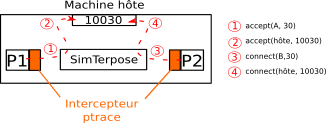
\includegraphics[scale=0.8]{Pictures/png/Mediation_realite}
    \caption{Communications réelles}
  \label{COMM_REALITE}
  \end{subfigure}
  \begin{subfigure}{0.25\textwidth}
  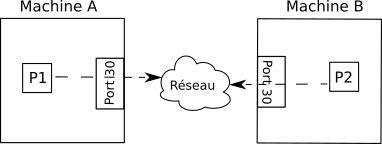
\includegraphics[scale=0.5]{Pictures/png/Mediation_VM}
  \caption{Communications vues \\ par les processus}
  \label{COMM_VM}
  \end{subfigure}
  \caption{Les communications réseaux entre deux processus}
  \label{COMM}
\end{figure}

De plus on ne peut pas se baser uniquement sur le numéro de \textit{file
  descriptor} associé à une socket pour identifier deux entités qui communiquent
entre elles. En effet ce \textit{file descriptor} est unique pour chaque socket
d'un processus, mais plusieurs processus peuvent avoir un même numéro de
\textit{file descriptor} pour des sockets de communications différentes puisque
chacune à son propre espace mémoire. Pour pallier à ce problème on va utiliser
en plus du numéro de socket, les adresses IP et les ports locaux et distants des
deux entités qui souhaitent communiquer comme moyen d'identification. Pour gérer
toutes ces modifications deux solutions ont été proposées lors d'un précédent
stage \citep{GUILLAUME:Interceptionsyscall}: la \textit{médiation par traduction
  d'adresse} et la \textit{full médiation}.

 \begin{figure}[H]
   \centering
   \begin{subfigure}{0.5\textwidth}
   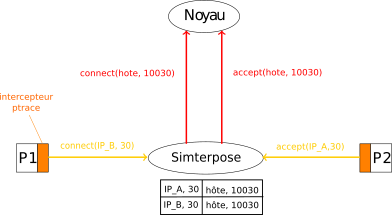
\includegraphics[scale=0.5]{Pictures/png/Mediation_translation_v2}
   \caption{Médiation par traduction d'adresse}
   \label{ADDRESS_TRANSLATION}
   \end{subfigure}
   \begin{subfigure}{0.4\textwidth}
     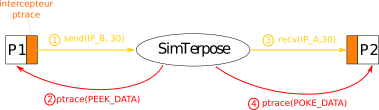
\includegraphics[scale=0.5]{Pictures/png/Mediation_full_v2}
  \caption{Full meditation}
  \label{FULL_MEDIATION}
   \end{subfigure}
   \caption{Les différents types de médiation}
   \label{MEDIATION}
 \end{figure}
 
\paragraph{Traduction d'adresse}
 Avec ce type de médiation, illustrée Fig.\ref{ADDRESS_TRANSLATION}, on considère
 que le noyau gère les communications. Ainsi en entrée et sortie d'appel système
 Simterpose va juste s'occuper de la transition entre le réseau virtuel simulé
 par SIMGRID et le réseau local, en utilisant les informations de communications
 contenues dans la socket. Pour cela, Simterpose gère un tableau de
 correspondances, dans lequel pour chaque couple <IP, ports virtuels> , on a un
 couple <IP, ports réels> associé.  De fait, en entrée d'un appel système de
 type réseau (\texttt{bind}, \texttt{connect}, \texttt{accept} ...), Simterpose
 doit remplacer l'adresse et les ports virtuels de l'application par l'adresse
 et les ports réels sur le réseau local, afin que la source de l'appel système
 corresponde à une machine existante sur le réseau local. Au retour de l'appel
 système, il faudra remodifier les paramètres en remettant l'adresse et les
 ports virtuels pour que l'application pense toujours être \textit{dans un
   environnement distribué.}  La limite de cette approche est liée au nombre de
 ports disponibles sur l'hôte.

\paragraph{Full médiation} 
Dans ce cas, le noyau ne va plus gérer les communications car nous allons
empêcher l'application de communiquer via des sockets et même d'établir des
connexions avec une autre application. Puisqu'il n'y a aucune communication, on
n'a pas besoin de gérer de tableau de correspondance d'adresse et de ports et
les applications peuvent conserver les adresses et les ports simulées qu'elles
considèrent comme réels. Quand l'application voudra faire un appel système de
type communication ou connexion vers une autre application, le processus espion
de Simterpose qui sera notifié via \texttt{ptrace} neutralisera l'appel système,
comme illustré sur la Fig.\ref{FULL_MEDIATION}. \textit{Ensuite, ce processus en
  utilisant \texttt{ptrace} récupérera, en lisant dans la mémoire du processus
  espionné, les données à envoyer ou récupérer et ira directement les lire ou
  les écrire dans la mémoire du destinataire.}  Même si la \textit{full
  médiation} permet d'éviter les communications réseaux et de conserver des
tables de correspondances, elle s'avère moins efficace dans le cas
d'applications qui communiquent énormément et utilisent de grosses données. En
effet, les appels à la mémoire sont bien plus coûteux que les communications
réseau.

 
%% begin{figure}
%%   \centering
%%   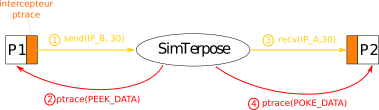
\includegraphics[scale=0.5]{Pictures/png/Mediation_full_v2}
%%   \caption{{\color{red} \textbf{TODO}}}
%%   \label{FULL_MEDIATION}
%% \end{figure}
